% !TeX program = xelatex
\documentclass[12pt,a4paper]{article}
\usepackage{fontspec}
\setmainfont{Times New Roman}
\usepackage[english,russian]{babel}
\usepackage{amsmath,amssymb,mathrsfs,cancel}
\usepackage[margin=22mm]{geometry}
\usepackage{graphicx,float}
\usepackage[unicode,hidelinks]{hyperref}
\DeclareMathOperator{\grad}{grad}
\DeclareMathOperator{\Div}{div}
\newcommand{\Rey}{\mathrm{Re}}
\setlength{\emergencystretch}{3em}
\interfootnotelinepenalty=10000
\newcommand{\topic}[1]{\par\medskip\noindent\textbf{#1}\par\nobreak\smallskip}
\renewcommand{\thefootnote}{\arabic{footnote})}
\begin{document}
\section*{Вопрос 6}
\noindent Гидравлическая теория безнапорной фильтрации. Уравнение Буссинеска. Формула Дюпюи для безнапорной фильтрации.

\medskip
\noindent\textbf{Источник:} Н. Е. Леонтьев. \textit{Основы теории фильтрации}. 2-е изд. Москва: МАКС Пресс, 2017. Глава II, § 9, печатные страницы 54--58.
\par\bigskip
% Источник: Leontiev-2017.pdf; печатная страница: 54; страница файла: 54
\section*{Глава II. Фильтрация несжимаемой жидкости в недеформируемой пористой среде}
\subsection*{§ 9. Гидравлическая теория безнапорной фильтрации}
\topic{Предположения гидравлической теории}
\setcounter{footnote}{0}
Строгое математическое описание безнапорных течений\footnote{Как уже говорилось на стр. 43, \textit{безнапорными} называются течения со свободной поверхностью.}, часто встречающихся в гидрологической практике, достаточно сложно из-за неизвестности формы поверхности депрессии. Для приближенного описания течений со свободной границей французским гидравликом и экономистом Жюлем Дюпюи [19] были предложены упрощающие предположения, которые выполняются для течений с \textit{пологой} поверхностью депрессии.
\setcounter{figure}{18}
\begin{figure}[H]\centering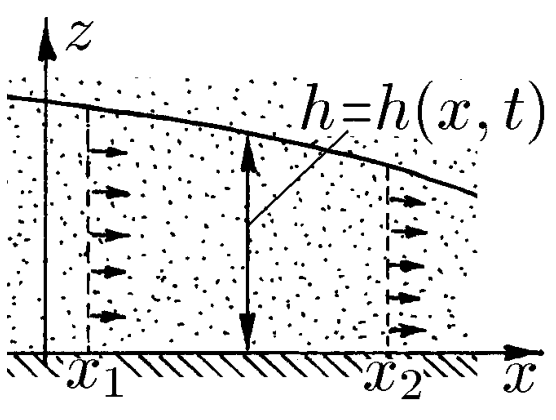
\includegraphics[width=.32\linewidth]{figures/figure-19.png}\caption{}\label{q6:fig-19}\end{figure}
Рассмотрим (для простоты плоское) нестационарное безнапорное течение несжимаемой жидкости в пористом слое, ограниченном снизу горизонтальной непроницаемой поверхностью (рис.~\ref{q6:fig-19}). Движение жидкости описывается уравнением неразрывности и законом Дарси, которые в показанной на рисунке системе координат имеют вид\footnote{Для сокращения записи мы будем иногда обозначать частные или обыкновенные производные штрихом, указывая переменную, по которой производится дифференцирование, с помощью нижнего индекса, например: $\frac{\partial p}{\partial x}=p'_x$.}
\begin{equation}\begin{gathered}
\frac{\partial u_x}{\partial x}+\frac{\partial u_z}{\partial z}=0,\qquad u_x=-C\frac{\partial}{\partial x}\left(\frac{p}{\rho g}+z\right)=-C\frac{p'_x}{\rho g},\\
u_z=-C\frac{\partial}{\partial z}\left(\frac{p}{\rho g}+z\right)=-C\left(\frac{p'_z}{\rho g}+1\right).
\end{gathered}\tag{9.1}\label{q6:eq-9-1}\end{equation}
Основное предположение гидравлической теории заключается в том, что при малых углах наклона свободной поверхности к горизонту ($h'_x\ll1$) в любом вертикальном сечении пласта $x=\mathrm{const}$ давление в фильтрующейся жидкости распределено по гидростатическому закону (что эквивалентно постоянству напора по сечению). Если эта гипотеза выполняется, то из закона Дарси следует,
% Источник: Leontiev-2017.pdf; печатная страница: 55; страница файла: 55
что скорость фильтрации в любой точке направлена горизонтально (ее вертикальная компонента равна нулю), а ее величина определяется только формой свободной поверхности и не зависит от высоты:
\[u_x(x,t)=-Ch'_x,\qquad u_z=0.\]
К указанной гипотезе можно прийти с помощью оценки членов в основных уравнениях. Поскольку мы хотим показать, что давление мало отличается от гидростатического, представим его в виде
\begin{equation}p(x,z,t)=\rho g(h(x,t)-z)+\widetilde p(x,z,t),\tag{9.2}\label{q6:eq-9-2}\end{equation}
где $\widetilde p$ --- отклонение от гидростатического закона. Обозначим характерные горизонтальные и вертикальные размеры смоченной части пласта через $L$ и $h$, характерное изменение высоты свободной поверхности --- через $\delta h$ (в силу предположения о пологости поверхности депрессии $\delta h/L\ll1$) и характерные проекции скорости фильтрации через $U_x$ и $U_z$. Тогда из уравнений \eqref{q6:eq-9-1}, в которые подставлено \eqref{q6:eq-9-2}, получаются оценки
\[\frac{U_x}{L}\sim\frac{U_z}{h},\quad U_x\sim\frac{C}{\rho g}\left(\rho g\frac{\delta h}{L}+\frac{\delta\widetilde p_x}{L}\right),\quad U_z\sim\frac{C}{\rho g}\cdot\frac{\delta\widetilde p_z}{h},\]
где $\delta\widetilde p_x$ и $\delta\widetilde p_z$ --- характерные изменения $\widetilde p$ вдоль соответствующих осей. Эти соотношения представляют собой оценки по порядку, и с ними можно обращаться как с обычными равенствами (возможно, если это потребуется, меняя коэффициенты при одночленах в конечное число раз)\setcounter{footnote}{0}\footnote{Скажем, от сравнения типа $\alpha\sim\frac34\beta-2\gamma$ можно перейти к сравнению $\alpha\sim\beta+\gamma$.}. Отсюда получается оценка
\[\rho g\delta h\sim\delta\widetilde p_x+\frac{L^2}{h^2}\delta\widetilde p_z,\]
из которой, в предположении, что $\delta\widetilde p_z$ по крайней мере не меньше $\delta\widetilde p_x$ (поскольку на свободной поверхности $\widetilde p=0$), а также $L\gtrsim h$, следует искомое соотношение
\[\delta\widetilde p_z\sim\rho gh\cdot\frac{h}{L}\cdot\frac{\delta h}{L}\ll\rho gh.\]
\topic{Уравнение Буссинеска}
С использованием предположений гидравлической теории легко получить уравнение для высоты свободной поверхности $h(x,t)$, записав закон
% Источник: Leontiev-2017.pdf; печатная страница: 56; страница файла: 56
сохранения массы для части пористой среды между двумя произвольными сечениями $x_1=\mathrm{const}$ и $x_2=\mathrm{const}$ (рис.~\ref{q6:fig-19}):
\[\begin{aligned}
\frac{d}{dt}\int_{x_1}^{x_2}\rho mh\,dx&=\left.(\rho h\cdot Ch'_x)\right|_{x_1}^{x_2}=\left.\rho C\left(\frac{h^2}{2}\right)'_x\right|_{x_1}^{x_2}\\
&=C\rho\int_{x_1}^{x_2}\left(\frac{h^2}{2}\right)''_{xx}\,dx,
\end{aligned}\]
откуда получается нелинейное \textit{уравнение Буссинеска} (J. Boussinesq, 1904)
\begin{equation}\frac{\partial h}{\partial t}=\frac{C}{2m}\frac{\partial^2(h^2)}{\partial x^2}.\tag{9.3}\label{q6:eq-9-3}\end{equation}
В общем случае зависимости высоты свободной поверхности от \textit{двух} пространственных координат в горизонтальной плоскости уравнение для $h=h(x,y,t)$ выглядит аналогично:
\[\frac{\partial h}{\partial t}=\frac{C}{2m}\triangle(h^2).\]
В частном случае стационарных течений форма поверхности депрессии находится из уравнения Лапласа
\[\triangle(h^2)=0.\]
\topic{Формулы Дюпюи для безнапорных течений}
В случае стационарного плоскопараллельного течения уравнение Буссинеска дает для формы свободной поверхности зависимость
\begin{equation}h^2(x)=Ax+B,\qquad A,B=\mathrm{const}\tag{9.4}\label{q6:eq-9-4}\end{equation}
\begin{figure}[H]\centering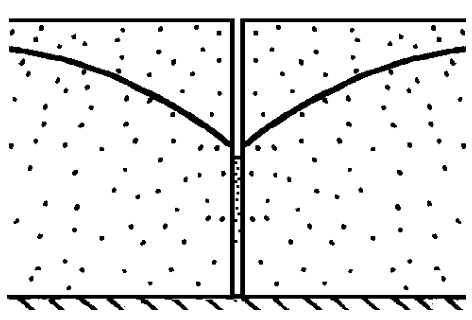
\includegraphics[width=.25\linewidth]{figures/figure-20.png}\caption{}\label{q6:fig-20}\end{figure}
(для течения слева направо, показанного на рис. 19, $A<0$), для которой постоянный объемный расход жидкости (на единицу длины в поперечном направлении)
\[Q=-Ch'(x)\cdot h(x)=-C(h^2(x)/2)'_x=-CA/2.\]
Записав \eqref{q6:eq-9-4} для двух сечений $x_1$ и $x_2$, несложно получить выражение расхода через высоты свободной поверхности в этих точках:
\begin{equation}Q=\frac{C}{2}\frac{h^2(x_1)-h^2(x_2)}{x_2-x_1}.\tag{9.5}\label{q6:eq-9-5}\end{equation}
% Источник: Leontiev-2017.pdf; печатная страница: 57; страница файла: 57
Аналогичным образом для стационарного осесимметричного безнапорного течения получим решение
\[h^2(r)=A\ln\left(\frac{r}{r_0}\right),\quad A,r_0=\mathrm{const}\]
с расходом
\[Q=-Ch'(r)\cdot2\pi rh(r)=-2\pi rC(h^2(r)/2)'_r=-\pi CA\]
(для притока к скважине, показанного на рис.~\ref{q6:fig-20}, $A>0$ и расход $Q$ отрицательный). Аналогично плоскому случаю, для расхода можно записать выражение
\begin{equation}Q=-\pi C\frac{h^2(r_2)-h^2(r_1)}{\ln(r_2/r_1)}.\tag{9.6}\label{q6:eq-9-6}\end{equation}
Соотношения \eqref{q6:eq-9-5} и \eqref{q6:eq-9-6} называются \textit{формулами Дюпюи} для пологой безнапорной фильтрации\setcounter{footnote}{0}\footnote{Сравните с формулой Дюпюи (7.5) на стр. 42.}.
\topic{Строгое доказательство формулы Дюпюи для фильтрации через прямоугольную плотину}
Формулы Дюпюи являются приближенными, т.к. при их выводе использовалась приближенная теория. Однако, что любопытно, в случае стационарной фильтрации через прямоугольную перемычку (рис.~\ref{q6:fig-21}) расход, определяемый по гидравлической теории, совпадает с точным значением, причем при любых (даже немалых) наклонах поверхности депрессии.
\begin{figure}[H]\centering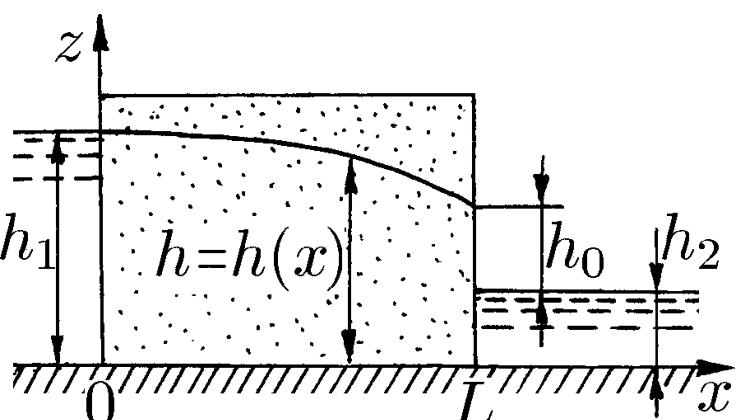
\includegraphics[width=.4\linewidth]{figures/figure-21.png}\caption{}\label{q6:fig-21}\end{figure}
Этот результат, полученный в 1951 г. И. А. Чарным, легко получается с помощью интегральных соотношений. В самом деле, постоянный расход жидкости с помощью закона Дарси выражается через давление
\[Q=\int_0^{h(x)}u_x(x,z)\,dz=-\frac{C}{\rho g}\int_0^{h(x)}p'_x(x,z)\,dz,\]
поэтому если ввести интеграл от давления по высоте
\[\mathscr{P}(x)\equiv\int_0^{h(x)}p(x,z)\,dz,\]
% Источник: Leontiev-2017.pdf; печатная страница: 58; страница файла: 58
то его производная явно вычисляется и оказывается равной константе:
\[\frac{d\mathscr{P}}{dx}=\cancel{p(x,h(x))}\cdot h'(x)+\int_0^{h(x)}p'_x(x,z)\,dz=-\frac{\rho gQ}{C}\]
(зачеркнутое слагаемое пропадает из-за равенства давления на свободной поверхности атмосферному давлению, которое мы полагаем нулевым). Поэтому функция $\mathscr{P}(x)$ является линейной, а ее значения на границах пласта вычисляются через известные параметры:
\[\mathscr{P}(x)=\mathscr{P}(0)-\frac{\rho gQ}{C}\,x,\]
\[\mathscr{P}(0)=\int_0^{h_1}\rho g(h_1-z)\,dz=\frac{\rho gh_1^2}{2},\quad
\mathscr{P}(L)=\int_0^{h_2}\rho g(h_2-z)\,dz=\frac{\rho gh_2^2}{2},\]
откуда получается выражение, совпадающее с \eqref{q6:eq-9-5}:
\[Q=\frac{C}{2}\frac{h_1^2-h_2^2}{L}.\]
Отметим, что если в этой задаче использовать гидравлическую теорию, то поверхность депрессии $h(x)$ должна выходить на правом конце пласта на значение $h_2$ (если мы хотим, чтобы в этой теории напор был непрерывен), тогда как в действительности выше поверхности воды имеется промежуток высачивания и $h(L)=h_2+h_0$.
% Конец § 9. Далее на странице 58 начинается § 10.

\end{document}
